\section{Question, scope and conventions}\label{sec:scope}
The paired-gap construction of Paper I provides a geometric setting for asking how a source state could be observed around an offset transverse circle.~\cite{PaperI} Paper II distinguishes that geometry from two additional comparison assumptions: a shared periodic carrier C1 and a passive exterior reception law C6.~\cite{PaperII} The present paper asks a computational question about a particular residual representation derived from those assumptions. How much of the timing of completed inputs survives in a compact state? Does its directional imbalance identify one pair, a history aggregate, or the last pair? What does coordinatewise saturation change?

Hilmir Frímann Halldórsson's motivation was to connect the paired construction and its observer responses to an explicit, testable temporal encoding. The investigations summarized here developed that question into a restricted event interface with matched Fourier and timestamp comparisons.~\cite{Pilot,Mechanism} A small state is useful only relative to a specified input and output contract. Neither a toroidal picture nor a successful subset of trials establishes general memory capacity.

We distinguish three objects: the exact lossless residual of C1; its finite-precision software representation; and a new, repeatedly projected numerical state. The third ceases to obey the first object's dynamics and work identity. The term SRG in retained empirical labels denotes the directional-coordinate implementation, not the native Tri-Octagon kernel or an entire family of character or memory systems. No native kernel, character-identity rule or physical receiver was evaluated in these comparisons.

The source record consists of the completed-pulse pilot and subsequent clipping-mechanism investigation, together with their internal mathematical/software reviews.~\cite{Pilot,Review09,Mechanism,Review10} The aligned majority formula and the clarification that the Fourier endpoint is an abstention are retained reviewer deductions. The proofs below state their hypotheses explicitly. Numerical results are the retained frozen comparisons; manuscript preparation introduces no new experimental corpus, performance measurement or decoder design.

\begin{table}[ht]
\centering\small
\begin{tabular}{P{30mm}P{119mm}}\toprule
Symbol & Meaning and convention\\\midrule
$L,c,T=L/c$ & Circumference, carrier speed and circuit time; $T$ is not a coordinate transform.\\
$\chi=s/R$ & Angle along the actual carrier circle, $L=2\pi R$.\\
$\epsilon=L/32$ & Source-tent arclength half-width, distinct from a physical shell or tube width.\\
$h,\rho$ & Height and radius of exterior arrays, retained from Papers I--II; never integer codes.\\
$\tau=t/T,\ d$ & Dimensionless analysis time and onset, common origin $\tau=0$.\\
$D,\phi$ & Pulse duration and common onset-phase offset; baseline $D=1$, aligned $\phi=0$.\\
$A,j$ & Nonnegative real source strength in $F_0$ units and port $j\in\{U,L\}$.\\
$\mu,z_U,z_L$ & Static mean and complex port moments in $F_0/c$ units.\\
$u_+,u_-$ & Directional amplitudes in the same units and global origin.\\
$\Mat,\Tp$ & Local complex matrix and real five-coordinate transform, not the native macro readout.\\
$b,H,\Delta$ & Bit width, numerical half-range and step $\Delta=2H/2^b$.\\
$K,\lambda,\upsilon$ & $K=2^{b-1}$ and integer endpoints $\lambda=-K,\ \upsilon=K-1$.\\
$(r,i)$ & Integer real/imaginary codes in a block; $i$ here is not $\ii=\sqrt{-1}$.\\
$\ell,N,D_N$ & Pair label, pair count and aligned count imbalance; $D_N$ is not duration.\\\bottomrule
\end{tabular}
\caption{Conventions separate geometry, time, source strengths and numerical storage. Geometric shell widths are not a quantizer step.}
\label{tab:conventions}
\end{table}

\section{Completed pulses and a five-real closure}\label{sec:closure}
\subsection{Inherited law and normalization}
On the circle, C1 is
\begin{equation}\label{eq:C1}
 p_t+c r_s=b_U(s)f_U(t)+b_L(s)f_L(t),\qquad r_t+c p_s=0,
\end{equation}
with zero preparation and periodic boundary conditions. Each $b_j$ is a translated unit-integral tent of half-width $\epsilon=L/32$. The paired contact angles and profile factors are
\begin{equation}\label{eq:geometry}
 \theta=\arctan(2/\sqrt3),\quad
 \chi_U=\pi-\theta,\quad\chi_L=\pi+\theta,\quad
 B_n=\sinc^2(n\pi/32),\quad \sinc x=\frac{\sin x}{x}.
\end{equation}
The circle, contact angle and exterior arrays are unchanged. Time normalization does not replace them by a unit-radius torus. Write $\widetilde p=cp/F_0$, $\widetilde r=cr/F_0$. An event is $f_j(t)=F_0 A h(\tau-d)$, where
\[
 h(q)=\sin^2(\pi q)\mathbf1_{[0,1]}(q),\qquad A\ge0 .
\]
It completes at $\tau=d+1$. Finite superpositions may overlap in time; closure is asserted only after all events have completed.

\begin{proposition}[Temporal moments and phase origin]\label{prop:moments}
For the positive temporal-transform convention, let
$I_n(d,A)=A\int_d^{d+1}h(\tau-d)e^{2\pi\ii n\tau}\dd\tau$.
Then $I_0=A/2$, $I_1=-Ae^{2\pi\ii d}/4$, $I_{-1}=\overline{I_1}$ and $I_n=0$ for integer $|n|\ge2$. A completed event adds
\begin{equation}\label{eq:event}
 z_e=-\frac{B_1A}{4}e^{-2\pi\ii d},\qquad
 \delta\mu=\frac A2,\qquad
 \delta u_\sigma=e^{\sigma\ii\chi_j}z_e,\quad \sigma=\pm1,
\end{equation}
with $u_\sigma$ referred to global normalized time zero.
\end{proposition}
\begin{proof}
Translate by $d$ and expand $h(q)=1/2-(e^{2\pi\ii q}+e^{-2\pi\ii q})/4$ on $[0,1]$. Orthogonality of integer exponentials gives the moments, including the negative sign. For an explicit sign check, the normalized characteristic field $(\widetilde p+\sigma\widetilde r)/2$ solves transport with source $LA b_jh/2$. Its spatial coefficient for $e^{-\sigma\ii\chi}$ is forced by $AB_1e^{\sigma\ii\chi_j}h/2$. The free factor is $e^{2\pi\ii\tau}$, hence variation of constants gives coefficient
$AB_1e^{\sigma\ii\chi_j}e^{2\pi\ii\tau}\int h(q-d)e^{-2\pi\ii q}\dd q/2$.
In the real-part convention that coefficient is $u_\sigma/2$, proving \eqref{eq:event} with the conjugate positive-time moment. The zero mode is $A/2$ since $T/L=1/c$ before normalization. The mean of $r$ remains zero by integrating its spatial derivative equation.
\end{proof}
A coefficient referred to $\tau_{\rm ref}$ multiplies $e^{2\pi\ii(\tau-\tau_{\rm ref})}$, so
\begin{equation}\label{eq:phase}
 u_\sigma^{(\tau_{\rm ref})}=e^{2\pi\ii\tau_{\rm ref}}u_\sigma^{(0)}.
\end{equation}
Paper II's one-period reference leaves it unchanged; its $3T/2$ reference multiplies it by $e^{3\pi\ii}=-1$. This conversion is common to both channels and every class. Reusing the latter coefficient at origin zero without this sign changes the waveform.

\begin{theorem}[Exact finite-family residual]\label{thm:closure}
For a finite superposition of completed events of the stated shape and duration, zero preparation and fixed contacts, define
\[
x=(\mu,\operatorname{Re}u_+,\operatorname{Im}u_+,\operatorname{Re}u_-,\operatorname{Im}u_-)\in\R^5
\]
by summing \eqref{eq:event}. After the last completion,
\begin{equation}\label{eq:residual}
 \begin{aligned}
 \widetilde p(\chi,\tau)&=\mu+\operatorname{Re}
 [(u_+e^{-\ii\chi}+u_-e^{\ii\chi})e^{2\pi\ii\tau}],\\
 \widetilde r(\chi,\tau)&=\operatorname{Re}
 [(u_+e^{-\ii\chi}-u_-e^{\ii\chi})e^{2\pi\ii\tau}].
 \end{aligned}
\end{equation}
No residual positive spatial mode above one remains. The coefficients need no update while sources are off.
\end{theorem}
\begin{proof}
The Fourier/characteristic solution of C1 is linear in its source. Each full event has zero temporal moment at every integer $|n|\ge2$, so its corresponding free residual coefficients vanish, even though the source tent has higher modes during forcing. The zero and first moments give \eqref{eq:residual}; finite superposition preserves it. The explicit free phase carries all subsequent motion. The stored amplitudes are therefore constant after completion. This proves the stated family closure, not a general forcing or active-event closure.
\end{proof}

\subsection{The interface is part of the claim}
A descriptor contains port, finite nonnegative onset, nonnegative amplitude and duration exactly one. It arrives at or after completion, in nondecreasing completion order. Zero amplitude changes neither coefficients nor timestamp validity; completion metadata may advance. A query requires a finite time at least the last completion and an explicit quiescent-batch promise. Five coordinates cannot detect an unseen active pulse. The implementation's unguarded algebraic \texttt{residual()} conversion is distinct from its guarded complete-state query.

Signal objects contain no raw history, pair ID, truth label, saved prior-state sequence or pending queue. The evaluator retains sorting, inputs and traces outside the encoder. Reset is explicit for independent pair trials; streams have no internal reset, subtraction, forgetting or normalization. Simultaneous descriptors supply no exact additive order feature. Nonlinear processing-order effects are separate and cannot manufacture temporal truth.

The timestamp comparator retains two last nonzero onsets, two validity flags and completion metadata. Nonoverlapping paired frames make these the final pair without pair IDs. It answers order and does not reconstruct fields. Raw-waveform acquisition and onset detection are outside all descriptor-input implementations.
\begin{figure}[ht]
\centering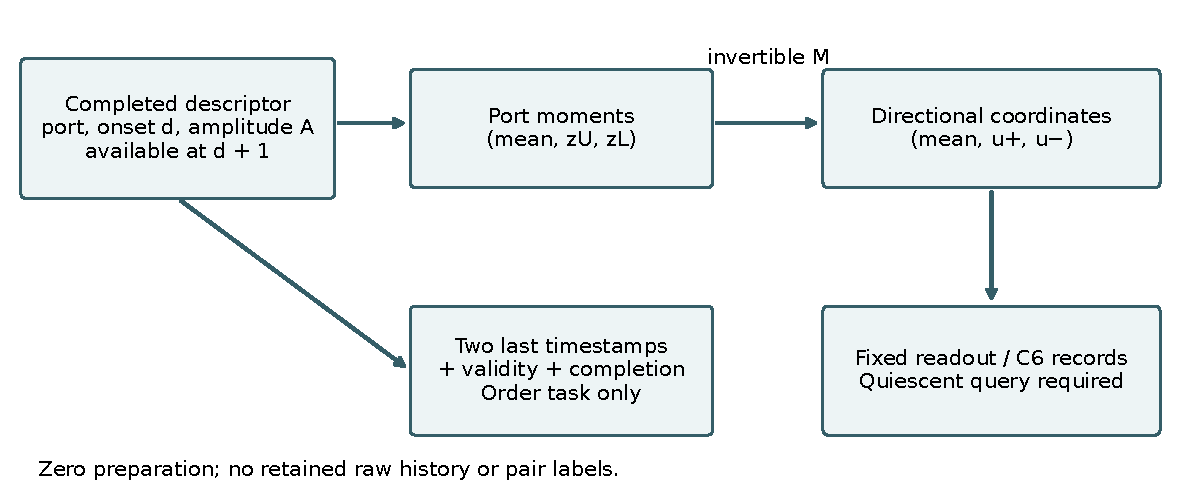
\includegraphics[width=\linewidth]{figures/fig01_interface.pdf}
\caption{Completed-event contract and exact basis equivalence. Arrows describe data access and algebra, not propagation in space. Completion and quiescence are required before exposing the residual.}
\label{fig:interface}
\end{figure}

\subsection{Storage, cross terms and the duration boundary}
The inherited normalized account and harmonic fraction are
\begin{equation}\label{eq:storage}
 \E(x)=\tfrac12\mu^2+\tfrac12|u_+|^2+\tfrac12|u_-|^2,\qquad
 \etaosc=\frac{|u_+|^2-|u_-|^2}{|u_+|^2+|u_-|^2}.
\end{equation}
The dimensional storage scale is $F_0^2L/c^2$. A zero harmonic denominator makes $\etaosc$ undefined. The total-storage fraction divides $(|u_+|^2-|u_-|^2)/2$ by $\E$, and is generally smaller in magnitude. For an additive increment $v$, expanding the square gives
\begin{equation}\label{eq:cross}
 \E(x+v)-\E(x)=x\cdot v+\tfrac12\norm v^2 .
\end{equation}
The account of a stream is not a sum of independent isolated-write accounts. C1's signed source-work law is conditional model mathematics, not native physical energy.

\begin{proposition}[Duration boundary and discarded tail]\label{prop:duration}
For $h_D(q)=\sin^2(\pi q/D)\mathbf1_{[0,D]}(q)$, $D>0$, put
$E(q,D)=(e^{2\pi\ii qD}-1)/(2\pi\ii q)$ for $q\ne0$ and $E(0,D)=D$. Then
\begin{equation}\label{eq:duration}
 I_n(D)=\tfrac12 E(n,D)-\tfrac14 E(n+D^{-1},D)-\tfrac14 E(n-D^{-1},D).
\end{equation}
For the retained two-unit-port stretched-pulse controls, the omitted normalized harmonic storage satisfies
\begin{equation}\label{eq:tail}
 \sum_{n>N}\E_n\le \frac{4\,32^4}{7\pi^6D^2N^7}.
\end{equation}
The omitted signed directional account has absolute value at most this bound.
\end{proposition}
\begin{proof}
Expansion of $\sin^2$ gives \eqref{eq:duration}, including the continuous zero-denominator values. Both $h_D$ and $h_D'$ vanish at the endpoints. Two integrations by parts give
$|I_n|\le(2\pi n)^{-2}\int_0^D|h_D''|\dd q$.
Here $h_D''=(2\pi^2/D^2)\cos(2\pi q/D)$, whose absolute integral is $4\pi/D$. Thus $|I_n|\le1/(\pi Dn^2)$. Each directional amplitude from two unit ports is bounded by $2B_n|I_n|$, regardless of onset/contact phases. Since $B_n\le32^2/(\pi^2n^2)$, its two-direction account is at most $4\,32^4/(\pi^6D^2n^8)$. Sum using $\sum_{n>N}n^{-8}\le\int_N^\infty x^{-8}\dd x=1/(7N^7)$. The absolute difference of nonnegative directional accounts is bounded by their sum.
\end{proof}
At $D=.98$ and $1.02$, the retained 70-digit evaluation through mode 512 gives discarded storage $5.24960914\,10^{-5}$ and $4.25775493\,10^{-5}$, with additional bounds $7.04\,10^{-17}$ and $6.50\,10^{-17}$. The first-mode projected fraction is $.989743319$ in both cases; full fractions are approximately $.989358003$ and $.989418686$. These are tail-qualified, non-interval decimal evaluations; the stated ratio reading allowance is $10^{-12}$, not a certified rounding enclosure. The primary API rejects both durations. Five coordinates then form only a projection, insufficient to synthesize the full carrier or exterior field.
